 % Opcje klasy 'iithesis' opisane sa w komentarzach w pliku klasy. Za ich pomoca
% ustawia sie przede wszystkim jezyk i rodzaj (lic/inz/mgr) pracy, oraz czy na
% drugiej stronie pracy ma byc skladany wzor oswiadczenia o autorskim wykonaniu.

\documentclass[declaration,shortabstract, mgr]{iithesis}
\usepackage{graphicx}
\usepackage[utf8]{inputenc}
\usepackage{url}

%%%%% DANE DO STRONY TYTUłOWEJ
% Niezaleznie od jezyka pracy wybranego w opcjach klasy, tytul i streszczenie
% pracy nalezy podac zarowno w jezyku polskim, jak i angielskim.
% Pamietaj o madrym (zgodnym z logicznym rozbiorem zdania oraz estetyka) recznym
% zlamaniu wierszy w temacie pracy, zwlaszcza tego w jezyku pracy. Uzyj do tego
% polecenia \fmlinebreak.
\polishtitle {System kontroli obecności na podstawie elektronicznych legitymacji studenckich}
\englishtitle {Students attendence verifing system with the use of student card}
\polishabstract {\ldots}
\englishabstract{\ldots}
% w pracach wielu autorow nazwiska mozna oddzielic poleceniem \and
\author {Dawid Szczyrk}
% w przypadku kilku promotorow, lub koniecznosci podania ich afiliacji, linie
% w ponizszym poleceniu mozna zlamac poleceniem \fmlinebreak
\advisor {dr Jakub Michaliszyn}
%\date {} % Data zlozenia pracy
% Dane do oswiadczenia o autorskim wykonaniu
%\transcriptnum {} % Numer indeksu
%\advisorgen {dr. Jana Kowalskiego} % Nazwisko promotora w dopelniaczu
%%%%%

%%%%% WLASNE DODATKOWE PAKIETY
%
%\usepackage{graphicx,listings,amsmath,amssymb,amsthm,amsfonts,tikz}
%
%%%%% WłaASNE DEFINICJE I POLECENIA
%
%\theoremstyle{definition} \newtheorem{definition}{Definition}[chapter]
%\theoremstyle{remark} \newtheorem{remark}[definition]{Observation}
%\theoremstyle{plain} \newtheorem{theorem}[definition]{Theorem}
%\theoremstyle{plain} \newtheorem{lemma}[definition]{Lemma}
%\renewcommand \qedsymbol {\ensuremath{\square}}
% ...
%%%%%

\begin{document}

\chapter{Wprowadzenie}

Celem niniejszej pracy jest zaprojektowanie użytecznego i niedrogiego w utrzymaniu systemu do kontroli obecności studentów na wykładzie.\\
\indent Niemalże każde zajęcia na naszym instytucie zaczynają się od zebrania listy obecności. Odbywa się to w siermiężny sposób, ponieważ każdy ze studentów musi wpisać swoje dane na listę obecności.
Taka forma jest uciążliwa, zajmuje kilka pierwszych minut zajęć, a studenci się rozpraszają podając sobie listę obecności. Dziś, kiedy do ochrony danych osobowych przykłada się
coraz większą wagę, starodawne sposoby sprawdzania obecności są tym bardziej wątpliwe.\\
\indent W dobie współczesnych zdobyczy technologicznych można uznać za zaskakujące, że wciąż trwamy przy tym czasochłonnym procesie. Wydawać by się mogło, że obecne podejście jest tak zakorzenione w akademickiej kulturze, że nie ma możliwości jego zmienić. Istnieją jednak opracowania które wskazują, że warto jest wdrażać nowoczesne rozwiązania, ponieważ ma to bezpośrednie przełożenie na prędkość sprawdzania obecności \cite{lcd}.\\
\indent Patrząc na problem sprawdzanie obecności z szerszej perspektywy. można również dojść do wniosku, że nie ma konieczności sprawdzania obecności w ogóle. Na studia w olbrzymiej części uczęszczają osoby dorosłe, odpowiedzialne za siebie, być moża należy wieć zrezygnować z kontroli. Zostało jednak sprawdzone \cite{theory_base}, że obecność ma wprost proporcjonalny wpływ na wyniki w nauce i odsetek uczniów porzucających studia przed ich ukończeniem. Wskazane zostało, że sprawdzanie obecności ma znaczenie nie tylko jako forma przymusu, ale również jako wyraz troski uczelni o swoich studentów i ma wpływ na ich morale\\\\
\indent Poniższa praca przedstawia proces od postawienia wymagań do realizacji finalnej wersji wielokomponentowego projektu. Na efekt ostateczny składają się aplikacje wykorzystujące najnowsze technologie i oparte na popularnych frameworkach, oraz niskopoziomowe elektroniczne urządzenie zaprojektowane i wykonane na potrzeby tego projektu.\\
\indent Z jednej strony w ramach pracy musiałem zaprojektować komunikację pomiędzy poszczególnymi komponentami, zaproponować i wdrożyć architekturę aplikacji internetowych, tzn. serwery na których wykonywany jest kod stron internetowych oraz bazy danych. W wersji finalnej użytkownikowi umożliwiono stworzenie własnego konta w internetowym serwisie i zarządzanie danymi o obecnościach w jego kontekście. Wszystko to zostało oparte na nowoczesnych rozwiązaniach chmurowych. \\
\indent Z drugiej strony moim zadaniem było zaprojektowanie niedrogiego urządzenia elektronicznego, które miało za zadanie udostępniać zrozumiały interfejs i realizować zadania związane ze zbieraniem danych od uczestników wykładu. Zagadnienie to wymaga wiedzy z zakresu elektroniki, zapoznania się ze schematami poszczególnych modułów oraz zrozumienia zasady ich działania. Kolejnym etapem projektu było połączenie odrębnych komponentów w jedną całość, a więc projekt układu elektronicznego na płytce stykowej i zamknięcie wszystkiego w opakowaniu umożliwiającym bezpieczne i wygodne użytkowanie.


\chapter{Analiza problemu}
\section{Przegląd obecnego sposobu sprawdzania obecności}
\indent W celu doprecyzowania wymagań stawianych przed projektowanym przeze mnie system postanowiłem rozważyć znany mi z autopsji proces weryfikowania obecności na zajęciach prowadzonych przez Uniwersytet Wrocławski\\
\indent Sprawdzanie listy obecności jest w dużej mierze uzależnione od preferencji prowadzącego i zwyczajów panujących na konkretnym wydziale - przykładowo obecność może być potwierdzona słownie - poprzez kolejne wywołanie osób z listy albo pisemnie - poprzez udostępnienie listy na którą uczestnicy będą zobowiązani się wpisać.\\
\indent Dla uproszczenia dalszych rozważań postanowiłem przyjąć za ogólnie stosowaną metodę pisemną - która według moich obserwacji jest stosowana częściej - i na tej podstawie wyodrębnić czynności które składają się na wypełnienie listy obecności podczas zajęć.\\
\indent Zbieranie informacji o obecności studentów na wykładzie jest czynnością na pierwszy rzut oka oczywistą, po bliższym przyjrzeniu się całej procedurze, okazuje się jednak, że daje się ona rozłożyć na jeszcze prostsze elementy. \\

\begin{itemize}
\item Przygotowanie kartki z listą obecności (przypisanie listy obecności do zajęć których będzie ona dotyczyła).
\item Udostępnienie kartki uczestnikom oraz wpisywanie się na listę.
\item Weryfikacja poprawności zebranej listy poprzez przeliczenie osób obecnych na zajęciach.
\item Przeniesienie zebranych danych do uczelnianego systemu.
\end{itemize}

\indent Powyższy schemat zbierania listy obecności podatny jest na dodatkowe błędy. Nie trudno wyobrazić sobie sytuację w której student intencjonalnie podał nie swoje dane w celu zaliczenia obecności innej osobie. Kolejnym krokiem który może doprowadzić do błędów na ostatecznej liście obecności jest błąd ludzki podczas przenoszenia danych z kartki do uczelnianego systemu komputerowego. Taki błąd trudno jest od razu wychwycić ze względu na to, że studenci zazwyczaj nie przeglądają na bieżąco list obecności dostępnych np. na USOSie. Kiedy na koniec semestru obecność jest rozliczana bardzo trudno dojść do faktów.\\
\indent Pierwszym elementem nadającym się w moim mniemaniu do usprawnienia jest samo tworzenie listy obecności z informację na temat zajęć których taka lista będzie dotyczyła. Fizyczna lista, poza czasem poświęconym na jej stworzenie, musi być po odbytych zajęciach przechowywana - co stwarza ryzyko jej zgubienia. Dodatkowo istnieje prawdopodobieństwo, że trafi w niepowołane ręce i ktoś nieżyczliwy wpisze na nią dodatkowe nazwiska. Do tego wszystkiego dochodzi jeszcze aspekt ekologiczny, ponieważ każda kolejna kartka generuje wymagające utylizacji śmieci. \\
\indent Również udział studentów w rejestrowaniu własnej obecności może ulec optymalizacji. Wpisanie własnego imienia i nazwiska, a czasem numeru albumu zabiera czas, naraża na upublicznienie dane osobowe i utrudnia studentowi śledzenie wykładu.\\
\indent Weryfikacja poprawności listy jest nie tylko pracochłonna, ale również podatna na błędy. Czas poświęcony na policzenie uczestników rośnie wprost proporcjonalnie do ich liczby. Dodatkowo prowadzący zajęcia może się zwyczajnie pomylić albo ktoś dopisać do listy już po tym sprawdzeniu.\\
\indent Z całą pewnością usprawnienia wymaga proces przenoszenia danych z fizycznego nośnika do uczelnianego systemu komputerowego. Problemem jest nie tylko to, że podczas wpisywania obecności do komputerowego systemu można popełnić błąd, ale również to, że jest to proces czasochłonny.\\

\section{Istniejące i możliwe realizacje zagadnienia}
\subsection{Podłączenie czytnika RFID bezpośrednio do komputera}
\indent Popularnym pomysłem usprawniającym system weryfikacji obecności jest skorzystanie technologii RFID (Radio-frequency identification). Wykorzystuje ona pole elektromagnetyczne do śledzenia na niewielkie odległości tagów (etykiet) RFID - małych transmiterów fal radiowych zdolnych do przechowywania danych umożliwiających zdalną identyfikację \cite{rfid_itself}. Tagi często mają formę kart, breloków lub innych łatwych w transporcie i przechowywaniu przedmiotów.\\
\indent W opracowaniu \cite{rfid_serial} przedstawiono projekt weryfikatora obecności zrealizowany przy pomocy radio technologii. Każdemu studentowi został przypisany tag z unikatowym identyfikatorem. System składa się z czytnika etykiet podłączonego do komputera przy użyciu portu szeregowego oraz aplikacji komputerowej, zdolnej do rozpoznawania zbliżonych do czytnika tagów i zapamiętywania którzy studenci zeskanowali swoje karty w trakcie zajęć. \\
\indent Ciekawym pomysłem przedstawionym w tym projekcie jest przekazanie osobnego tagu prowadzącemu zajęcia. Zbliżenie tej etykiety na początku i na końcu zajęć do czytnika wyznacza ramy czasowe podczas których obecność może zostać zaliczona studentom. Dodatkowo zastosowano tutaj podejście w którym uczestnik powinien rejestrować swoje pojawienie się jak i opuszczenie zajęć - jest to odstępstwo od tradycyjnej formy zbierania obecności. \\
\indent W projekcie można zaobserwować kilka wad. Wykorzystany czytnik RFID jest urządzeniem w całości dostarczonym przez producenta. Można spodziewać się że jest to rozwiązanie drogie, a samego urządzenia nie będzie dało się rozszerzyć o dodatkowe funkcjonalności. \\
\indent Taka architektura pociąga za sobą konieczność ciągłego połączenia z komputerem oraz dodatkowego okablowania. Może to powodować problemy logistyczne, jeśli chcielibyśmy korzystać z systemu w różnych salach.\\
\indent Sama aplikacja komputerowa katalogująca zebrane obecności również poddana jest ograniczeniom. Korzystanie z tego systemu możliwe jest wyłącznie na komputerach, na których zainstalowano taką aplikację, co jest rozwiązaniem uciążliwym. Baza danych zapamiętująca obecności współdzielona jest pomiędzy poszczególne instancje aplikacji na różnych komputerach, jest więc ona udostępniona publicznie, co ułatwia nieautoryzowany dostęp.

\subsection{Podłączenie przy pomocy kabla ethernetowego}
\indent W opracowaniu opisanym w pracy \cite{rfid_serial} zaproponowano podobną realizację, tym razem w oparciu o bezpośrednie podłączenie czytnika do internetu kablem RJ45. Wykorzystywane urządzenie jest stworzone na bazie Arduino Uno i rozszerzone o moduł RFID i gniazdo pozwalające podłączyć kabel ethernetowy. \\
\indent Zaproponowany projekt rozwiązuje problem konieczności korzystania z komputera w bezpośrednim połączeniu z czytnikiem, a wybrany układ elektroniczny pozwala rozszerzyć urządzenie o dodatkowe funkcjonalności. Łączność internetowa pozwala na natychmiastowe odnotowywanie obecności w bazie, co na pewno jest wygodnym rozwiązaniem. \\
\indent W treści opracowania nie został poruszony problem połączenia obecności z zajęciami na których została ona odnotowana. W przypadku rozszerzenia systemu o kolejne czytniki podłączone do sieci i korzystania z wielu urządzeń jednocześnie, nie będzie możliwości rozszyfrowania, z jakich zajęć pochodzą spływające do serwera dane. \\
\indent Jedynym możliwym sposobem na komunikację urządzenia z użytkownikiem, jest w tym wypadku buzzer, co może okazać się niewystarczające do wyrażenia stanu urządzenia. W razie kłopotów z łącznością albo anteną RFID, nie ma możliwości wygodnego sygnalizowania problemu.

\subsection{Samodzielny czytnik }
\indent W cytowanym we wstępie opracowaniu \cite{lcd}, w celu rozwiązania powyższego problemu zaproponowano wykorzystanie z wyświetlacza LCD, z którego użytek robi opisany w tej pracy układ elektroniczny. Przedstawione w pracy urządzenie poza czytnikiem RFID, zdolne jest również do wyświetlania treściwych komunikatów potwierdzających udane odnotowanie karty studenta. \\
\indent Trudno w tym wypadku dyskutować jednak z innymi rozwiązaniami technicznymi zawartymi w tej pracy, ponieważ motywem przewodnim tego opracowania jest pokazanie, że sprawdzanie obecności przy pomocy tagów RFID przebiega szybciej niż w klasycznym podejściu.

\subsection{Aplikacja internetowa umożliwiająca rejestrowanie obecności studentów na zajęciach przez internet lub telefon}
\indent W mojej ocenie to najprostsze rozwiązanie składające się z jednolitego systemu, w którym jednocześnie można zbierać obecności uczestników wykładu, oraz je przechowywać i przeglądać. Jej niewątpliwym plusem jest całkowite wyeliminowanie problemu związanego z wprowadzaniem danych do systemu katalogującego obecności, ponieważ dane wprowadzane są wprost do systemu. Identyfikacja konkretnych zajęć w ramach których rejestrowana jest obecność, odbywałaby się na początku zajęć poprzez wejście w kontekst odpowiedniego wykładu w aplikacji. Obecność uczestników na zajęciach byłaby sprawdzana przez prowadzącego i od razu wprowadzana do systemu. \\
\indent Nie zdecydowałem się na to rozwiązanie, ponieważ wydaje mi się ono nieszczególnie odbiegać od aktualnej procedury, poza zmianą nośnika z kartki papieru na ekran tabletu.

\subsection{Urządzenie rejestrujące obecności za pośrednictwem sieci bezprzewodowej}
\indent To rozwiązanie początkowo wydało mi się bardzo atrakcyjne i przez długi czas miałem zamiar je zrealizować. Planowałem rozszerzyć mikrokontroler o moduł do bezprzewodowej łączności z internetem i w stworzonej aplikacji udostępnić interfejs do odnotowywania obecności. \\
\indent Po dłuższych rozważaniach okazało się jednak, że takie rozwiązanie przerasta moje możliwości. Ten sposób wysyłania danych do aplikacji katalogującego obecności wymagałby umożliwienia powiązania obecności z zajęciami, na których zostały zebrane \\
\indent Wymagałoby to dołączenia dodatkowego interfejsu który pozwalałby wprowadzać takie dane, co jeszcze bardziej komplikowałoby projektowane przeze mnie urządzenie. Dodatkowo ograniczyłoby to zbiór układów scalonych z których mógłbym skorzystać, ponieważ musiałbym wybrać takie, które posiadają wystarczającą ilość pamięci, pinów i innych potrzebnych peryferiów. \\
\indent Ostatecznie moje plany dotyczące takiego projektu pokrzyżował moduł ESP, który miał realizować komunikację bezprzewodową, ale okazał się bardzo kapryśny.

\section{Określenie wymagań wobec projektu}
\indent W poprzednim rozdziale wspomniano o wielu możliwych realizacjach problemu zbierania obecności, co jest i tak tylko niewielkim wycinkiem możliwych do wykonania projektów. W opracowaniu \cite{review} wspomniano o wielu innych przedsięwzięciach, z których na wspomnienie zasługują na pewno:

\begin{itemize}
\item Skorzystania z telefonu komórkowego i łączności bluetooth w celu odnotowania obecności.
\item Wykorzystanie odcisku palca do dodatkowego potwierdzenia tożsamości studenta.
\item Użycia kamery i rozpoznawania twarzy w celu identyfikacji wchodzących na wykład studentów.
\end{itemize}

\indent Analiza powyższych rozwiązań wraz z ich mocnymi i słabymi stronami pozwoliła wyłonić zbiór wymagań wobec projektowanego systemu. Wymagania zostały dobrane pod kątem poprawienia wydajności klasycznego sposobu weryfikowania obecności, co zostało rozważone w rozdziale 2.1, oraz możliwości jakie dają współczesne technologie - które zostały opisane powyżej.

\subsubsection{Urządzenie powinno udostępniać następujące funkcjonalności':}

\begin{enumerate}
\item Zarejestrowanie obecności uczestnika zajęć przy pomocy tagu RFID.
\item Wyświetlanie jasnych komunikatów odnośnie stanu urządzenia.
\item Powiązanie obecności z zajęciami, podczas których zostały zebrane.
\item Potwierdzenie tożsamości uczstnika odnotowującego swoją obecność.
\item Katalogowanie zebranych danych i generowanie raportów podsumowujących.
\item Wygodne przeniesienie obecności zebranych przez czytnik do aplikacji przechowującej dane.
\end{enumerate}



\chapter{Określenie struktury projektu}
\indent Finalnie zdecydowałem, żeby jednoznacznie oddzielić sposób zbierania danych od ich przechowywania i przetwarzania.\\
\indent W realizacji projektu skorzystałem z faktu, że polskie uczelnie powszechnie korzystają z Elektronicznych Legitymacji Studenckich (ELS), które zawierają wbudowany tag RFID. \\
\indent Komponent umożliwiający studentowi odnotowanie swojej obecności na wykładzie - weryfikator - postanowiłem oprzeć o platformę Arduino - znaną mi z zajęć systemów wbudowanych. Urządzenie zostało rozszerzone o moduły umożliwiające realizację założeń z poprzedniego rozdziału. \\
\indent Czytnik fal radiowych umożliwiający odczytanie danych z etykiety RFID znajdującej się na ELS. Gniazdo USB pozwalające podłączyć pendrive na którym zostaną przeniesione dane z urządzenia na bazie Arduino do aplikacji internetowej przechowującej dane. \\ 
\indent Dodatkowo częścią urządzenia będzie zegar RTC umożliwiający zapamiętanie godziny, o której odnotowane zostały obecności, a więc powiązanie ich z konkretnymi zajęciami, oraz wyświetlacz LCD + Buzzer, pozwalające na wygodne korzystanie z samodzielnego urządzenia. \\
\indent Sposobem na potwierdzenie tożsamości studenta, będzie w wypadku realizowanego projektu porównanie zdjęcia na legitymacji z twarzą osoby która zbliża ją do czytnika. Za tę weryfikację odpowiedzialny będzie prowadzący.\\\\

\indent Rolę oprogramowania odpowiedzialnego za katalogowanie zebranych przez weryfikator danych będzie pełnić w moim systemie ogólnodostępna aplikacja internetowa, umożliwiająca założenie konta i zarządzanie zebranymi obecnościami w kontekście całego przedmiotu i w kontekście pojedynczych zajęć. Dodatkowo ma ona umożliwiać generowanie raportów ze zagregowanymi danymi, tak aby dało się łatwo prześledzić obecności w kontekście całego semestru. \\
\indent Postanowiłem uczynić realizowany projekt niezależnym od danych studentów. Dzięki takiemu podejściu w łatwy sposób będę mógł przełączyć cały system na korzystanie z baz danych na różnych uczelniach oraz uniknę konieczności przechowywania wrażliwych danych w systemie. \\
\indent Ze względu na to, że na etapie realizowania założonego projektu nie uzyskałem dostępu do serwisu udostępniającego dane wrocławskich studentów, stworzyłem własną, niezależną od innych części projektu, aplikację realizującą funkcję bazy danych studentów. \\
\indent Umożliwia ona powiązanie danych pobranych z legitymacji studenckiej z danymi pozwalającymi na jego identyfikację. Jest to aplikacja rozłączna względem systemu zarządzającego obecnościami osób uczestniczących w zajęciach, wystawiająca RESTowe api.

\chapter{Realizacja}
\section{Weryfikator - czytnik legitymacji studenckich}
\indent Zgodnie z wymaganiami projektowane przeze mnie urządzenie powinno udostępniać co najmniej następujące możliwości.
\begin{itemize}
\item Możliwość podłączenia zewnętrznego nośnika danych.
\item Stworzenie pliku na którym zapamiętani zostaną uczestnicy zajęć
\item Zebranie informacji z elektronicznej legitymacji studenckiej, potwierdzające obecność uczestników
\item Wyświetlanie informacji o stanie urządzenia, w szczególności sukcesu odczytania danych z legitymacji
\item Zapamiętanie czasu kiedy zebrane zostały obecności
\end{itemize}
\indent Dodatkowo, chciałbym żeby cała elektronika schowana była wewnątrz plastikowego opakowania, a zasilanie dostarczane za pomocą kabla podłączonego do sieci elektrycznej. Opakowanie powinno zostać wyposażone w otwory na kabel zasilający, zewnętrzny nośnik danych, wyświetlacz. Czytnik kart RFID powinien być tak zlokalizowany aby umożliwić łatwe zebranie danych z ELS.
\subsection{Zastosowana platforma i peryferia}
\indent Arduino to cała platforma programistyczna umożliwiająca łatwe projektowanie i testowanie układów składających się z wielu elektronicznych modułów. Podstawą każdego projektu Arduino jest układ elektroniczny oparty na mikroprocesorze. Pod egidą tego systemu udostępniony jest cały wachlarz wersji takich układów, różniących się rodzajem kontrolera i udostępnionymi peryferiami (przykładowo: slot na kartę SD, gniazdo RJ-45, wbudowany wyświetlacz, czy moduł WIFI). Do wyboru użytkownika pozostaje cała gama wersji płytek drukowanych spod znaku Arduino. Dodatkowo platforma udostępniona jest na licencji open hardware, co sprawiło, że z projektem związana jest olbrzymia międzynarodowa społeczność entuzjastów elektroniki. Częścią platformy jest również środowisko programistyczne umożliwiające wgrywanie własnych programów na podłączoną do komputera płytkę.\\
\indent Ciekawą opcją dostępną dla użytkowników platformy jest możliwość skonstruowania własnej płytki z procesorem na bazie powszechnie dostępnych schematów gotowych układów. Może to być rozwiązanie bardzo atrakcyjne w przypadku kiedy projektantowi zależy na ograniczeniu kosztów układu. W moim rozwiązaniu postanowiłem nie iść tak daleko i skorzystać z jednej z gotowych płytek.\\
\indent Podstawą mojego weryfikatora postanowiłem uczynić płytkę Arduino Uno oparte na mikroprocesorze AVR ATmega328. Kontroler w tym układzie jest bardzo prosty, posiada bardzo mocno ograniczone zasoby, co wymusza dodatkowy wysiłek włożony w zarządzanie pamięcią i czasem procesora. Do mojej dyspozycji miałem następujące zasoby\\
\begin{itemize}
\item 32kB Flash - przestrzeń na kod programu
\item 2kB SRAM zajmowane przez pamięć operacyjną.
\item porty SPI, I2C, szeregowy
\item Jednostka obliczeniowa o częstotliwości zegara 20MHz
\end{itemize}
\indent Dodatkowo, w celu zapewnienia wszystkich wymaganych funkcjonalności przez projektowany przeze mnie weryfikator, skorzystałem z następujących dodatkowych modułów:
\begin{itemize}
\item Czytnik RFID - do odczytywania danych z legitymacji studenckiej wyposażonej w interfejs zbliżeniowy. Czytnik podłączony jest przez port szeregowy
\item USB Host Shield - dodające gniazdo USB, umożliwiające podłączenie pendriva, korzystający z drugiego portu SPI
\item Wyświetlacz LCD wraz z potencjometrem do ustawiania kontrastu, przekazujący użytkownikowi informacje na temat stanu urządzenia
\item RTC - zegar czasu rzeczywistego z baterią do zapamiętywania czasu zbierania danych, korzystający z interfejstu I2C
\item Buzzer piezo wydający dźwiękowe sygnały w razie sukcesu
\end{itemize}
\subsection{Konstrukcja}
\indent Do skonstruowania ostatecznego układu z zebranych elementów używam dodatkowo:
\begin{itemize}
\item Jednej dwustronnej płytki stykowej
\item Dwóch rezystorów 220 Ohm
\item kilkudziesięciu kabli różnej długości
\item Jednego przycisku do resetowania zegara
\end{itemize}
\indent Cały układ został osadzony w plastikowym opakowaniu z wywierconymi otworami\\
\begin{figure}[h]
\caption{Układ elektroniczny}
\centering
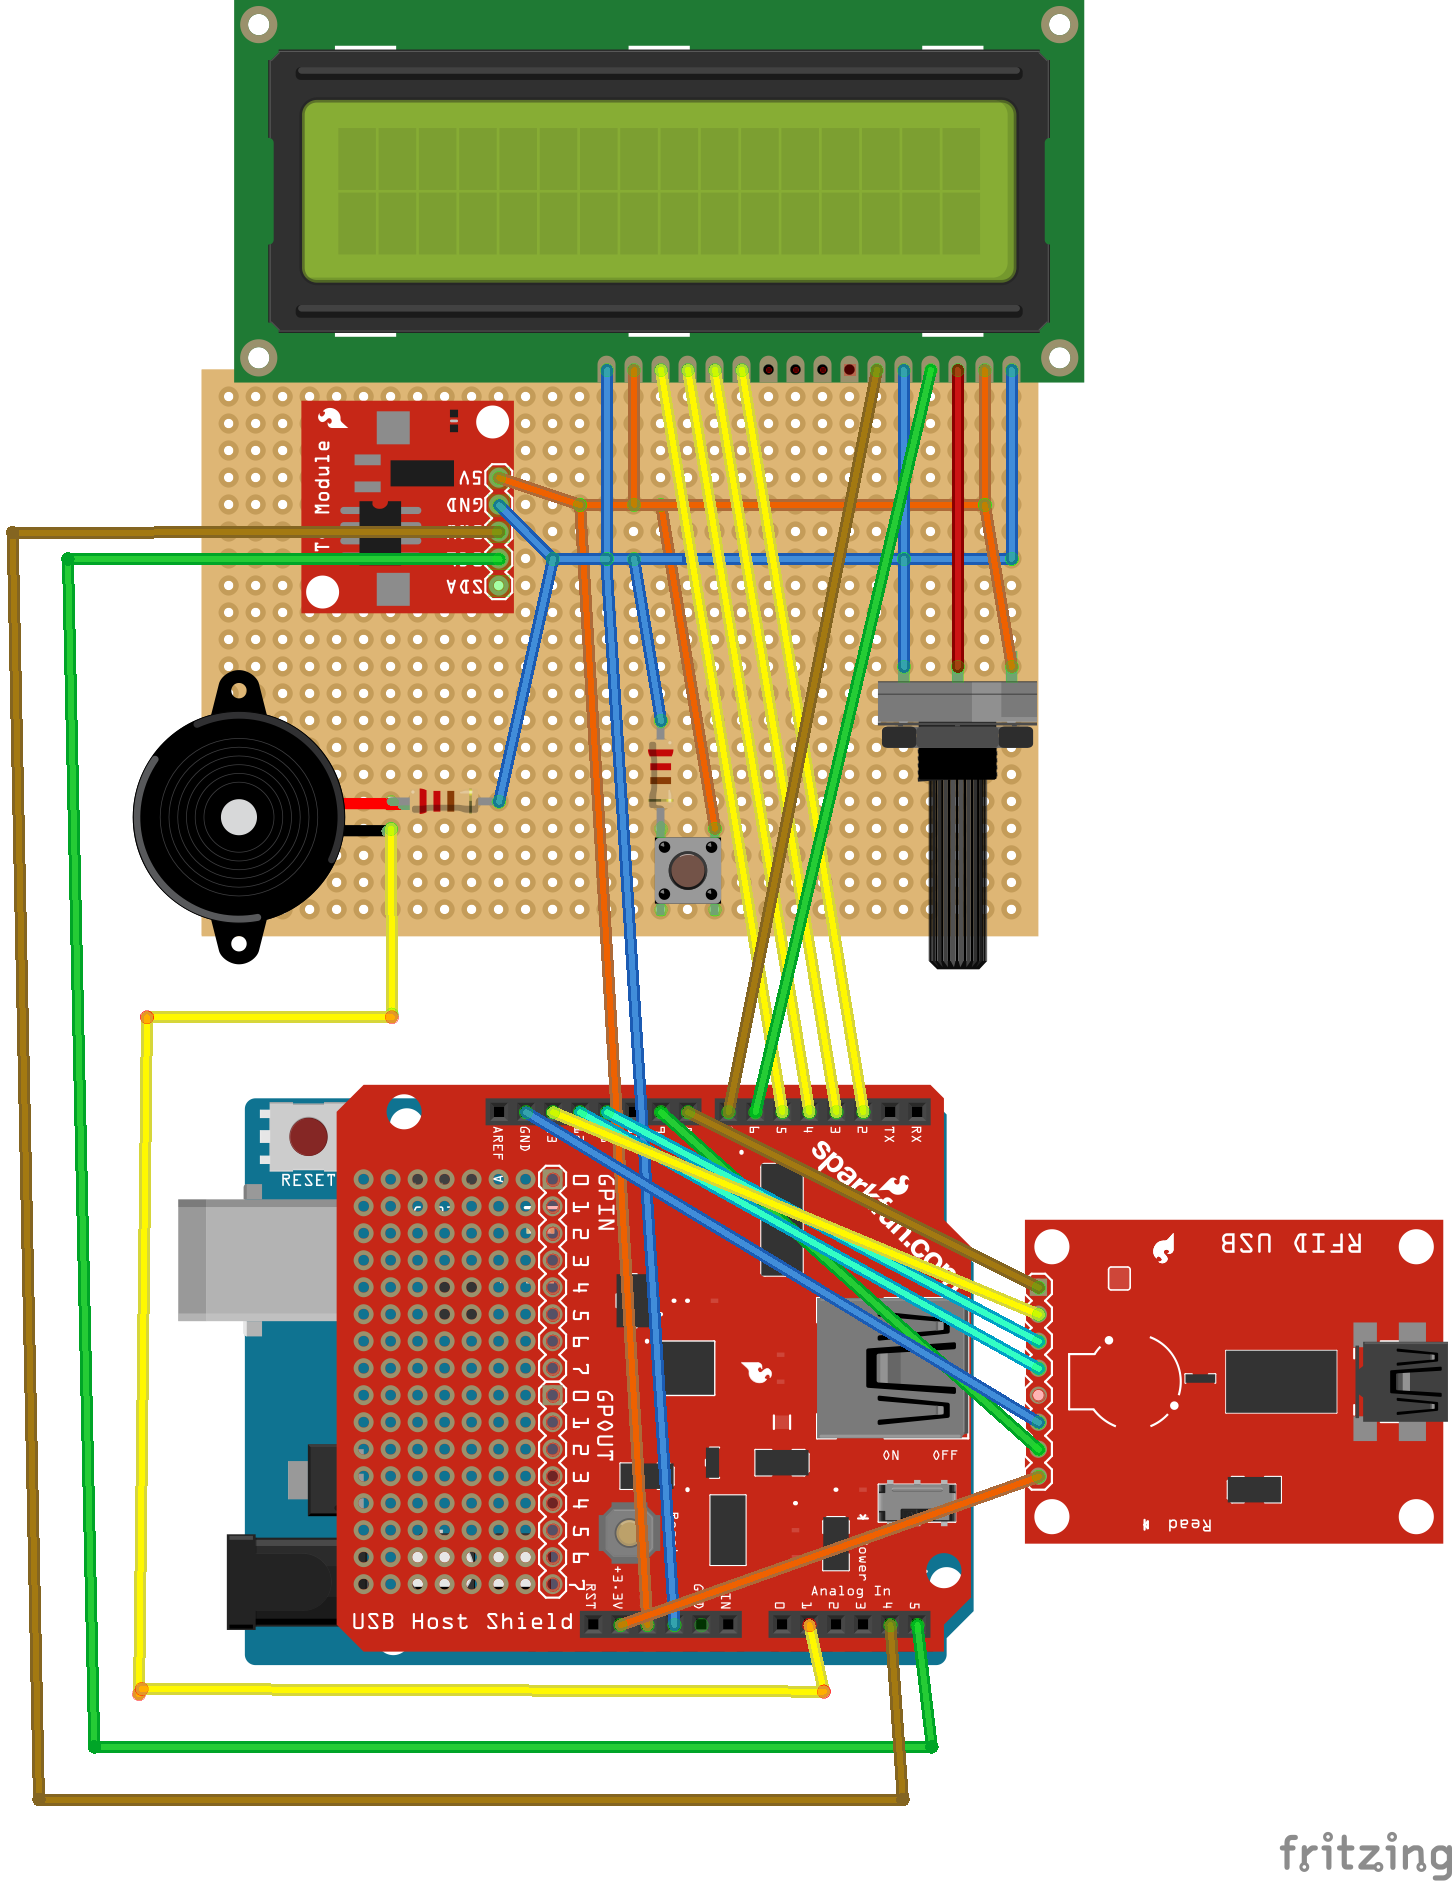
\includegraphics{circuit.png}
\end{figure}
\subsection{Działanie}
\indent Osią działania zaprojektowanego przeze mnie weryfikatora jest interakcja z dwoma zewnętrznymi urządzeniami. Jednym z nich jest nośnik danych na którym zapisane zostaną obecności uczestników zajęć. W realizowanym projekcie rolę tę pełni pendrive sformatowany w systemie FAT. W zależności od tego czy w danym momencie pendrive jest podłączony, urządzenie jest w stanie oczekiwania na drugie z zewnętrznych narzędzi - Elektroniczną Legitymację Studencką. Dodatkowo weryfikator jest zdolny do wyświetlanie komunikatów o swoim stanie na ekranie LCD i wydawania sygnałów dźwiękowych przy pomocy brzęczka. Częścią urządzenia jest również zegar RTC, który pozwala śledzić aktualną godzinę. Weryfikator monitoruje swój własny stan i jest zdolny do wykrywania błędów takich jak:
\begin{itemize}
\item Błąd Inicjalizacji podłączonego pendrive'a
\item Błąd zapisu odczytanych danych na nośniku
\item Błąd zegara RTC - spowodowanego najczęściej rozładowaną baterią
\end{itemize}
\indent Kod mojego weryfikatora projektowałem z myślą o tym, żeby łatwo dało się przedstawić przebieg programu na diagramie. Struktura kodu jest przemyślana w taki sposób, żeby podczas jednego przebiegu pętli głównej wykonywał się jedynie kod powiązany z aktualnym stanem urządzenia. Taki układ nie tylko pozwala zwięźle opowiadać o działaniu urządzenia, ale również ułatwia testowanie poprawności podczas pisania kodu i montowania urządzenia.\\
\indent Weryfikator w danej chwili może znajdować się w jednym z 12 stanów. Na przedstawionym diagramie stany oczekujące na zdarzenie przedstawiono kolorem kremowym, a stany przejściowe kolorem niebieskim:
\begin{figure}[h]
\caption{Diagram stanów}
\centering
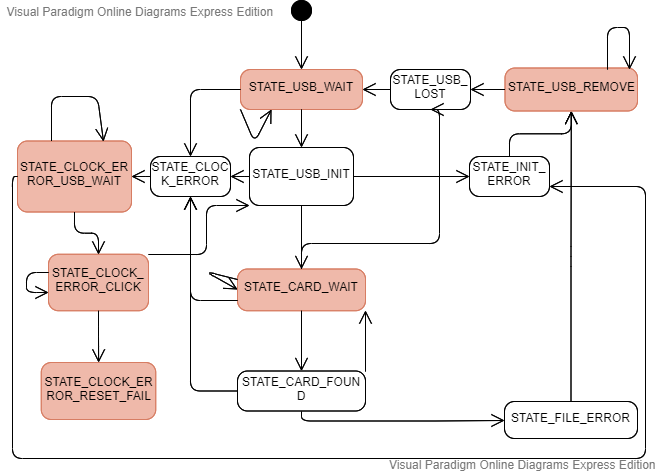
\includegraphics[scale=0.6]{state_machine.png}
\end{figure}

\begin{itemize}
\item STATE\_USB\_WAIT - oczekiwanie na pendrive - ekran wyświetla informację - "Insert pendrive". Próba inicjalizacji nośnika zajmuje około 5 sekund dlatego wyświetlany czas jest aktualizowany z opóźnieniem
\item STATE\_USB\_INIT - inicjalizacja pendriva - po odnalezieniu pendriva wyświetlana jest informacja "USB Inserted". W przypadku błędu inicjalizacji - przejście do stanu STATE\_INIT\_ERROR, w razie sukcesu na podstawie aktualnego czasu stworzona i zapamiętana zostaje nazwa YY-MM-DD-hh\_mm\_ss dla pliku który będzie przechowywał zebrane uidy. STATE\_CARD\_WAIT.
\item STATE\_CARD\_WAIT - oczekiwanie na kartę RFID - ekran: "Scan Card". W razie wykrycia odłączenia pendriva przejście do stanu STATE\_USB\_LOST. W przypadku wykrycia karty, ale błędu w odczycie (np. ze względu na zbyt szybkie odsunięcie karty) wyświetlenie informacji: Read error.
\item STATE\_CARD\_FOUND - zapisywanie Uidu do pliku - otwarcie pliku o zapamiętanej nazwie zapisanie do niego odczytanego Uidu. W razie błędu przy zapisie przejście do stanu STATE\_FILE\_ERROR, w przypadku sukcesu sygnał dźwiękowy, wyświetlenie informacji "Read Success" i powrót do stanu STATE\_CARD\_WAIT
\item STATE\_INIT\_ERROR - błąd inicjalizacji pendriva - ekran: "Init Error"
\item STATE\_USB\_REMOVE - czekanie na odłączenie pendriva. Wyświetlacz:''Reinsert USB". W razie wykrycia odłączenia pendriva przejście do stanu STATE\_USB\_LOST.
\item STATE\_USB\_LOST - odłączono pendrive . Ekran: "USB removed", sygnał dźwiękowy oraz przejście do stanu STATE\_USB\_WAIT
\item STATE\_FILE\_ERROR - błąd zapisu do pliku. Ekran: ''Open file error", przejście do stanu STATE\_USB\_REMOVE
\item STATE\_CLOCK\_ERROR - błąd zegara - w razie wykrycia problemów z zegarem w którymś ze stanów [STATE\_USB\_WAIT, STATE\_CARD\_WAIT, STATE\_CARD\_FOUND, STATE\_USB\_INIT, STATE\_USB\_REMOVE] sterowanie przechodzi do tego stanu. Wyświetlona zostaje informacja: "Clock Error", następnie sterowanie przechodzi do STATE\_CLOCK\_ERROR\_USB\_WAIT
\item STATE\_CLOCK\_ERROR\_USB\_WAIT - oczekiwanie na pendrive z czasem - wyświetlacz "Insert pendrive with time". Sterowanie pozostaje w tym stanie do czasu kiedy na zewnętrznym nośniku wykryty zostanie plik o nazwie tdav, który w pierwszym wierszu będzie zawierał datę w formacie "YYYY/MM/DD hh:mm:ss". W przypadku wykrycia poprawnego pliku program zapamiętuje datę z pliku tdav i przechodzi w stan STATE\_CLOCK\_ERROR\_CLICK\\
- W razie błędu przy inicjalizacji pendriva program przechodzi do stanu STATE\_INIT\_ERROR \\
- W razie wykrycia pendrive i nie wykrycia pliku o nazwie tdav wyświetlona zostaje informacja "Upload time tdav"\\
- W razie złego formatu pierwszej linijki w pliku tdav wyświetlona zostaje informacja: "Bad date format"
\item STATE\_CLOCK\_ERROR\_CLICK - oczekiwanie na reset. Wyświetlacz: "Click to reset". Sterowanie pozostaje w tym stanie do czasu kiedy zostanie przyciśnięty guzik resetu. Po naciśnięciu guzika na zegarze zostaje ustawiona zapamiętana data, wyświetlony zostaje komunikat "Time set", a sterowanie przechodzi w stan STATE\_USB\_INIT. Jeśli podczas ustawiania czasu na zagarze wystąpi błąd program przechodzi w stan STATE\_CLOCK\_ERROR\_RESET\_FAIL \\
\item STATE\_CLOCK\_ERROR\_RESET\_FAIL - błąd resetowania czasu. Wyświetlacz: ''Clock Reset Fail". Ze względu na brak możliwości ustawienia poprawnego czasu jest to stan, z którego urządzenie nie może wrócić do poprawnego funkcjonowania.
\end{itemize}
\subsection{Procedura resetowania zegara RTC}

\subsection{Napotkane problemy}
\subsubsection{Dwa moduły korzystające z interfejsu SPI}
\indent Początko zamiast Arduino Uno planowałem użyć innej wersji tej popularnej płytki - Arduino Leonardo. \\
\indent Tak jak w wersji którą ostatecznie zrealizowałem, planowałem do układu Leonardo podłączyć USB Host Shield oraz moduł RFID - oba używają interfejsu SPI. Każdy z tych komponentów osobno współpracował poprawnie z Arduino Leonardo. Problemy pojawiły się kiedy próbowałem podłączyć wszystko w jedną całość i zapisywać odczytane dane z karty magnetycznej na podłączonym pendrivie. \\
\indent Podczas montowania układu problemem nie do przeskoczenia okazało się to, że w przypadku tej wersji płytki piny interfejsu SPI znajdują się w magistrali ICSP, która jest zajęta przez moduł USB w taki sposób, że nie ma możliwości podłączyć tam innych kabli. \\
\indent Próbowałem jeszcze dolutować kable do magistrali CSP na płytce USB Host Shield, jednak ze względu na to że, są to jedynie milimetrowe wypustki, przepaliłem któreś z połączeń wewnątrz tego układu i ostatecznie musiałem je wyrzucić. \\
\indent W celu rozwiązania problemu z portem SPI przeszedłem na wersję UNO które interfejs SPI ma doprowadzony również na piny 10-13. \\

\subsubsection{Problemy z odczytaniem danych z ELS}
\indent W początkowej wersji urządzenie korzystało z modułu RFID - MFRC-522. Ten komponent bez zarzutów współpracował z załączonymi w zestawie tagami, jednak bardzo słabo wykrywał Elektroniczną Legitymację Studencką. Odczytanie Uidu z ELS zajmowało zazwyczaj parę minut. Żeby rozwiązać ten problem postanowiłem zamienić moduł RFID, na taki o którym czytałem, że ma lepszy zasięg - PNS532. Pierwsze próby zwiastowały pełny sukces - próby odczytania danych z ELS przebiegały bez zarzutu. \\
\indent Problem pojawił się jednak przy współpracy nowego modułu z resztą układu. Jak już zostało wcześniej wspomniane, Arduino Uno posiada jeden port SPI, do którego można podłączyć więcej urządzeń. Niestety w tym wypadku rzeczywistość okazała się odbiegać od oczekiwań. Arduino było w stanie współpracować tylko z jednym z dwóch komponentów - albo USB Host shield albo modułem PNS532. Ostatecznie okazało się jednak, że moduł PNS532 udostępnia również inne porty, dzięki czemu udało mi się go podłączyć przy pomocy portu szeregowego.
\begin{figure}[h]
\caption{Uklad USB Host shield ze wskzaniem na zakończenia magistrali CSP}
\centering
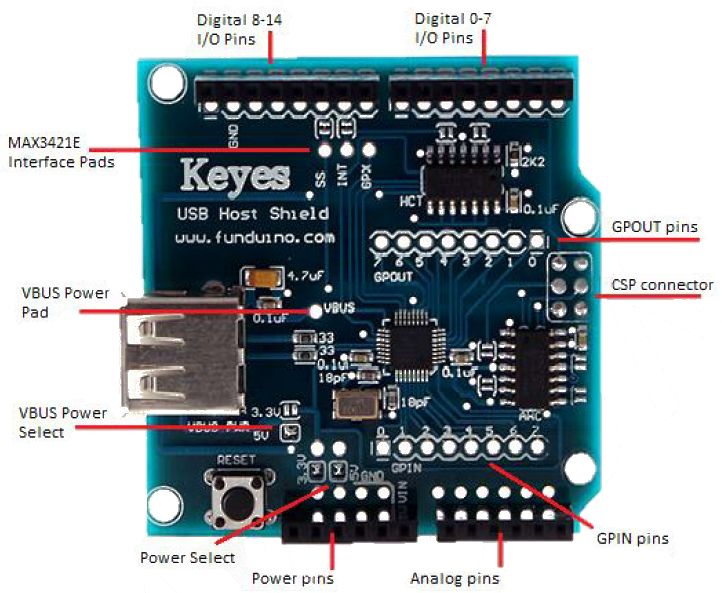
\includegraphics[scale=0.6]{usb_host_shield.jpg}
\end{figure}

\subsubsection{Wypełniona pamięć operacyjna}
\indent W miarę dołączania kolejnych komponentów do układu, tzn. zegara RTC, brzęczka oraz wyświetlacza LCD, zacząłem natrafiać na problemy z pamięcią. \\
\indent Pierwsza skończyła się pamięć operacyjna której mój kontroler posiadał jedynie 2KB. Objawiało się to nagłym zawieszaniem się wykonywania programu, co w pierwszym momencie było dla mnie zaskakujące i niezrozumiałe.\\
\indent Udało mi się rozwiązać ten problem dzięki większej dyscyplinie w korzystaniu z pamięci. Ograniczyłem liczbę zmiennych globalnych, a największy efekt przyniosło przeniesienie wykorzystywanych w programie napisów z pamięci operacyjnej do pamięci flash, do czego służy dyrektywa PROGMEM.\\
\indent Pamięć flash jest przeznaczona do przechowywania kodu programu i nie ma do niej swobodnego dostępu jak w przypadku pamięci operacyjnej. Dodanie kolejnej biblioteki która ułatwiłaby przechowywanie danych w tej przestrzeni nie było możliwym ze względu na ograniczone zasoby.\\
\indent Ostatecznie zdecydowałem się na korzystanie z pamięci flash wczytując dane bajt po bajcie. Chcąc więc wyświetlić komunikat na ekranie LCD, tak czy inaczej musiałem najpierw wczytać bajtowo łańcuch znaków do pamięci operacyjnej, jednak nie było już potrzeby przechowywać wszystkich łańcuchów znaków jednocześnie w SRAM.
\begin{figure}[h]
\caption{Stałe programu przechowywane w pamięci flash}
\centering
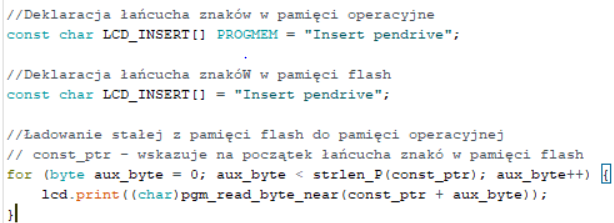
\includegraphics[scale=0.8]{progmem.png}
\end{figure}
\subsubsection{Wypełniona pamięć flash}
\indent Przeniesienie łańcuchów znaków do pamięci flash, chociaż poprawiło wydajność pamięci operacyjnej, to spowodowało wyczerpanie przestrzeni przeznaczonej na kod programu. \\
\indent Pamięć flash jest bardziej pojemna niż SRAM ponieważ w tym wypadku jest to aż 32KB do dyspozycji programisty, jednak duża liczba bibliotek do obsługi peryferiów doprowadziła do wyczerpanie się również tej przestrzeni. \\
\indent Ułatwieniem w przypadku optymalizowania wykorzystania pamięci flash jest to, że przestrzeń zajmowana przez kod programu jest stała po kompilacji. Nie ma więc obawy że w trakcie przebiegu programu nastąpi nagły wzrost i przekroczenie pojemności. Wystarczy dostosować się do limitu 32 KB. \\
\indent Udało mi się tego dokonać poprzez ograniczenie liczby funkcji które deklarowałem w moim programie, oraz schowanie komunikatów wysyłanych na serial monitor wewnątrz dyrektyw preprocesora \#if DEBUG serial.println(''SETUP"); \#endif. Dzięki temu mogłem łatwo wyłączyć kod programu odpowiedzialny za debugowanie.\\
\subsubsection{Moduł WIFI}
\indent W pierwszej wersji planowanego przeze mnie weryfikatora, miał on się łączyć z siecią za pomocą modułu WIFI. Bardzo dużo kłopotów sprawił mi jednak układ ESP8266, odpowiedzialny za tę łączność. Po wgraniu sterownika do tego układu przestawał on być wykrywany przez komputer i Arduino.\\ 
\indent Pomimo wykorzystania kilku takich układów za każdym razem pojawiał się ten sam problem. Nie udało mi się dociec jaka była tego przyczyna. Ostatecznie odszedłem od wykorzystania modułu ESP8266 ze względu na zmianę koncepcji.
\subsection{Inne koncepcje weryfikatora}
\indent Zastanawiając się nad ostateczną formą jaką powinien przyjąć projektowany przeze mnie weryfikator brałem jeszcze pod uwagę układ Raspberry Pi. Ostatecznie zrezygnowałem z tego pomysłu, ze względu na to że takie urządzenie mogłoby wymagać utrzymywania systemu operacyjnego aktualnej wersji. Za wykorzystaniem Arduino przemawia również cena takiego układu i fakt, że jest on mi bardzo dobrze znany z zajęć Systemów Wbudowanych.\\
\indent Projektując układ musiałem również podjąć decyzję z jakiego nośnika skorzystać do przenoszenia danych z weryfikatora do aplikacji zarządzającej obecnościami. Brałem pod uwagę dwie możliwości. Poza opcją na którą się ostatecznie zdecydowałem, brałem jeszcze pod uwagę korzystanie z kart SD \\
\indent Ze względu na większą dostępność i łatwiejsze podłączenie klasycznego pendrive'a do komputera ( nie każdy komputer posiada slot na kartę SD), zdecydowałem się nie tę właśnie możliwość. Później okazało się, że ta decyzja miała swoje konsekwencje.\\
\indent Po pierwsze USB Host Shield zajął magistralę ICSP, będącą jedynym wyjściem pinów interfejsu SPI w układzie Arduino Leonrado. Po perypetiach wcześniej już przeze mnie opisanych, zdecydowałem się na zmianę wersji płytki na Uno. \\
\indent Kolejnym utrudnieniem które zostało postawione na mojej drodze ze względu na korzystanie z pendriva, były problemy z dostępnością biblioteki obsługującej pamięć w tej formie. Podstawowa biblioteka obsługująca układ USB Host Shield nie przewiduje wykorzystania złącza USB do podłączenia pamięci masowej. \\
\indent Ostatecznie udało mi się znaleźć nieszczególnie popularną bibliotekę do obsługi tego narzędzia - UsbFat, która jednak okazała się być słabo opisana.
\section{Menedżer obecności - umożliwiający katalogowanie danych}
\section{Baza studentów - umożliwiająca identyfikację danych zebranych z ELS}

\chapter{Możliwość dalszego rozwoju systemu}
\subsubsection{Zautomatyzowana weryfikacja}
\indent Mankamentem zaprezentowanego w powyższej pracy podejścia jest konieczność manualnej weryfikacji czy osoba zbliżająca legitymację do czytnika jest rzeczywiście jej właścicielem. W opracowaniu \cite{fingerprint}, przedstawiono projekt udostępniania informacji o studencie w oparciu o kartę RFID oraz dodatkową weryfikację poprzez sprawdzenie linii papilarnych. W systemie weryfikującym obecność na zajęciach można byłoby skorzystać z podobnego rozwiązania.\\
\indent Innym dającym się zastosować podejściem jest system do rozpoznawania twarzy.
\subsubsection{Integracja z uczelnianym systemem}
\indent Projektowany przeze mnie system od początku pomyślany był w taki sposób, aby umożliwić integrację z zewnętrznym źródłem informacji o studentach. Bazę studentów, która w moim projekcie jest osobną aplikację, łatwo można by zastąpić przez akademicką platformę. Kolejnym polem do integracji jest system logowania. Korzystanie z konta z USOSa, byłoby ułatwieniem dla korzystających z aplikacji pracowników i studentów oraz pozwoliłoby uniknąć przechowywania w systemie wrażliwych danych związanych z utworzonymi kontami.
\subsubsection{Udostępnienie systemu uczestnikom wykładu}
\indent Rozwinięciem systemu byłoby na pewno udostępnienie studentom funkcjonalności zalogowania się i wglądu do ich aktualnych statystyk związanych z obecnościami. Byłoby to zadanie o tyle utrudnione, że należałoby udostępniać zainteresowanemu dane dotyczące tylko jego osoby. Można byłoby to rozwiązać poprzez integrację z uczelnianym systemem do logowania albo udostępniając studentom konta zakładane przez administratora, który zajmowałby się potwierdzeniem tożsamości.
\subsubsection{Informowanie zainteresowanych o obecnościach}
\indent W cytowanym we wstępie opracowaniu \cite{theory_base} wskazane jest, że sprawdzanie obecności ma znaczenie nie tylko jako forma przymusu, ale również jako wyraz troski uczelni o swoich studentów. Wskazane jest, że `wczesna interwencja` w przypadku opuszczania przez ucznia zajęć, może zapobiec przerwaniu przez niego studiów. Nasuwa to bardzo wiele możliwości rozwoju aplikacji weryfikującej obecności. Zaprojektowaną przeze mnie platformę można by wyposażyć w możliwość informowania studenta o tym, że limit jego nieobecności na pewnych zajęciach jest bliski wyczerpania się. \\
\indent Możliwe również byłoby automatyczne informowanie organów uczelnianych o kłopotach studenta na podstawie jego absencji. \\
\subsubsection{Platforma do szybkiego reagowania}
\indent Idąc tym tropem, integrując uczelniane systemy, udostępniając studentom wgląd w ich obecności i umożliwiając interakcje poprzez kanały takie jak mail czy sms, można z prostej aplikacji stworzyć rozbudowaną platformę do monitorowania wyników studenta i adekwatnego reagowania w przypadku wykrycia potencjalnych problemów. Powiązując informacje na temat tego na jakim etapie studiów znajduje się student z jego aktualnymi wynikami, byłoby możliwe automatyczne dopasowanie pomocy, takiej jak rozmowa z pracownikiem uczeni odpowiedzialnym za studentów, czy zaproponowanie dodatkowych zajęć

\chapter{Wnioski}

\ldots

\begin{thebibliography}{9}
	\bibitem{theory_base}
		Debbie Bevitt and Chris Baldwin and Jane Calvert,
		\textit{Intervening Early: Attendance and Performance Monitoring as a Trigger for First Year Support in the Biosciences}
		2016, Bioscience Education
		\url{https://doi.org/10.3108/beej.15.4}
	\bibitem{bluetooth}
		Vishal Bhalla and Tapodhan Singla and Ankit Gahlot and Vijay Gupta
		\textit{Bluetooth Based Attendance Management System}
		2013
		\url{http://citeseerx.ist.psu.edu/viewdoc/summary?doi=10.1.1.645.1573}
	\bibitem{ethernet}
		Oo, Zaw Lin and Win Lai, Theint and Than, Maung Maung
		\textit{Web Server Base RFID Attendance Record Systems}
		2018
		\url{https://www.researchgate.net/publication/333115623_Web_Server_Base_RFID_Attendance_Record_System/comments}
	\bibitem{review}
		Patel, Unnati and Swaminarayan, Priya
		\textit{Computer Science and Management Studies Development of a Student Attendance Management System Using RFID and Face Recognition: A Review}
		2014, International Journal of Advance Research in Computer Science and Management Studies
		\url{https://www.researchgate.net/publication/325819350_Computer_Science_and_Management_Studies_Development_of_a_Student_Attendance_Management_System_Using_RFID_and_Face_Recognition_A_Review}
	\bibitem{rfid_serial}
		Arulogun, Oladiran and Olatunbosun, Adeboye and A., Fakolujo and Olayemi Mikail, Olaniy
		\textit{RFID-Based Students Attendance Management System}
		2013, International Journal of Engineering and Scientific Research
		\url{https://www.researchgate.net/publication/235598499_RFID-Based_Students_Attendance_Management_System}
	\bibitem{lcd}
		Shoewu, Oluwagbemiga and Makanjuola, N. and Ajasa, Abiodun and Oluwafemi J., Ayangbekun
		\textit{Design and Implementation of an Rfid Based Automated Students Attendance System R BASAS}
		2015, JOURNAL OF ADVANCEMENT IN ENGINEERING AND TECHNOLOGY
		\url{https://www.researchgate.net/publication/235598499_RFID-Based_Students_Attendance_Management_System}
	\bibitem{rfid_itself}
		\url{https://en.wikipedia.org/wiki/Radio-frequency_identification}
\end{thebibliography}
\end{document}
